\documentclass[a4paper,12pt]{article}

\usepackage[utf8]{inputenc}
\usepackage{geometry}
\usepackage{graphicx}
\graphicspath{{Figures/}}
\usepackage{mathptmx}
\usepackage{setspace}
\usepackage{titlesec}
\usepackage{parskip}
\usepackage{indentfirst}
\usepackage{listings}
\usepackage{xcolor}
\usepackage{hyperref}

\lstset{
    breaklines=true,
    postbreak=\mbox{\textcolor{red}{$\hookrightarrow$}\space},
}

\setlength{\parindent}{1em}

\definecolor{dkgreen}{rgb}{0,0.6,0}
\definecolor{gray}{rgb}{0.5,0.5,0.5}
\definecolor{mauve}{rgb}{0.58,0,0.82}
\definecolor{dkblue}{rgb}{0,0,0.5}
\definecolor{lightblue}{rgb}{0,0.5,0.8}
\definecolor{darkred}{rgb}{0.6,0,0}
\definecolor{backcolour}{rgb}{0.97,0.97,0.97}

\lstdefinestyle{javastyle}{
    language=Java,
    backgroundcolor=\color{backcolour},   
    commentstyle=\color{dkgreen}\itshape,
    keywordstyle=\color{dkblue}\bfseries,
    stringstyle=\color{mauve},
    basicstyle=\ttfamily\footnotesize,
    breakatwhitespace=false,         
    breaklines=true,                 
    captionpos=b,                    
    keepspaces=true,                 
    numbers=left,                    
    numbersep=5pt,                  
    showspaces=false,                
    showstringspaces=false,
    showtabs=false,                  
    tabsize=4,
    frame=lines,
    rulecolor=\color{gray},
    moredelim=[s][\color{orange}]{@}{\ },
}

\lstdefinestyle{xmlstyle}{
    language=XML,
    backgroundcolor=\color{backcolour},
    basicstyle=\ttfamily\footnotesize,
    morekeywords={xmlns,version,type,scope,groupId,artifactId,dependencies,dependency,project,modelVersion,build,plugins,plugin,configuration,source,target},
    keywordstyle=\color{darkred}\bfseries,
    commentstyle=\color{dkgreen}\itshape,
    stringstyle=\color{dkblue},
    tagstyle=\color{darkred},
    breaklines=true,
    numbers=left,
    numbersep=5pt,
    tabsize=2,
    frame=lines
}

\geometry{
    top=3cm,
    left=4cm,
    right=3cm,
    bottom=3cm
}

\renewcommand{\thesection}{\Alph{section}} 

\renewcommand{\thesubsection}{\thesection.\arabic{subsection}}

\titleformat{\section}
  {\normalfont\Large\bfseries}
  {\thesection.}
  {1em}
  {}

\begin{document}

\begin{titlepage}
    \centering
    \onehalfspacing

    {\fontsize{14}{17}\selectfont \textbf{LAPORAN PRAKTIKUM}} \\[0.2cm]
    {\fontsize{16}{19}\selectfont \textbf{PRAKTIKUM PENGUJIAN PERANGKAT LUNAK}} \\[0.5cm]
    {\fontsize{14}{17}\selectfont \textbf{PERTEMUAN 1}} \\[0.2cm]
    {\fontsize{14}{17}\selectfont \textbf{JUNIT}}
    
    \vfill
    
\includegraphics[width=6cm]{Figures/UGM.png} 
    \vfill
    
    {\large Disusun Oleh:} \\[0.5cm]
    
    \begin{tabular}{l c l} 
        Nama & : & Abdullah Afif Habiburrohman \\
        NIM  & : & 537611/SV/24441 \\
        Kelas & : & BB / B2 \\
        Dosen & : & Divi Galih Prasetyo Putri, S.Kom., M.Kom., Ph.D.
    \end{tabular}
    
    \vfill
    
    {\fontsize{12}{14}\selectfont \textbf{
        PROGRAM STUDI SARJANA TERAPAN \\ 
        TEKNOLOGI REKAYASA PERANGKAT LUNAK \\
        DEPARTEMEN TEKNIK ELEKTRO DAN INFORMATIKA \\
        SEKOLAH VOKASI \\
        UNIVERSITAS GADJAH MADA \\
        YOGYAKARTA \\
        2026
    }}
    
\end{titlepage}

\tableofcontents
\newpage

\section{Dasar Teori}

Dalam pengembangan perangkat lunak berbasis Java, pengelolaan pustaka (library) dan dependensi sering kali menjadi tantangan tersendiri jika dilakukan secara manual. Apache Maven hadir sebagai alat otomatisasi build dan manajemen proyek yang menggunakan konsep Project Object Model (POM). Inti dari konfigurasi Maven terletak pada file pom.xml, di mana pengembang dapat mendefinisikan struktur proyek serta dependensi eksternal yang dibutuhkan.

\begin{sloppypar}
Pengujian perangkat lunak dilakukan secara bertingkat, dan tingkatan paling dasar dalam hierarki ini adalah unit testing. Fokus utama dari pengujian ini adalah memverifikasi unit terkecil dari perangkat lunak untuk memastikan bahwa unit tersebut menghasilkan keluaran yang benar sesuai dengan masukan yang diberikan. Penerapan unit testing sejak awal pengembangan bertujuan untuk mengidentifikasi kesalahan logika lebih dini sehingga perbaikan dapat dilakukan dengan biaya yang lebih rendah serta meningkatkan kualitas kode secara keseluruhan.

JUnit merupakan salah satu kerangka kerja (framework) pengujian yang paling populer dalam ekosistem Java. JUnit menyediakan mekanisme standar untuk menulis dan menjalankan pengujian otomatis yang dapat diulang (repeatable), sehingga validasi kode dapat dilakukan terus-menerus selama siklus pengembangan.

Berbeda dengan versi pendahulunya yang bersifat monolitik, JUnit 5 (generasi terkini) dibangun dengan arsitektur modular yang terdiri dari tiga sub-proyek utama:

\begin{enumerate}
    \item JUnit Platform: Berfungsi sebagai fondasi untuk meluncurkan kerangka kerja pengujian di JVM. Ini adalah komponen yang memungkinkan IDE (seperti IntelliJ IDEA) untuk mendeteksi dan menjalankan tes.

    \item JUnit Jupiter: Merupakan model pemrograman dan ekstensi baru untuk menulis tes dan ekstensi di JUnit 5. Ini menyediakan anotasi modern seperti @Test, @BeforeEach, serta metode asersi.

    \item JUnit Vintage: Menyediakan mesin uji untuk menjalankan tes yang ditulis menggunakan JUnit 3 dan JUnit 4 demi kompatibilitas ke belakang.
\end{enumerate}

Dalam implementasi praktisnya, sering kali membingungkan untuk menentukan dependensi mana saja yang perlu dimasukkan (apakah hanya API, Engine, atau Params). Oleh karena itu, tersedia artefak bernama JUnit Jupiter (Aggregator).

Inti dari sebuah pengujian unit adalah verifikasi, yang dalam JUnit dilakukan melalui mekanisme Assertion. Asersi mendefinisikan kondisi yang dianggap benar; jika kondisi tersebut terpenuhi, maka tes dianggap lulus (pass), dan jika tidak, tes dianggap gagal (fail).

JUnit menyediakan berbagai metode statis untuk keperluan ini, antara lain:

\begin{enumerate}
    \item assertEquals: Membandingkan kesesuaian antara nilai yang diharapkan (expected) dengan nilai aktual yang dihasilkan kode.

    \item assertTrue: Memastikan sebuah kondisi bernilai benar.

    \item assertNotNull dan assertNull: Memeriksa keberadaan objek (apakah null atau tidak).
\end{enumerate}

Selain itu, untuk menangani skenario pengujian yang kompleks, JUnit Jupiter menyediakan metode assertAll. Metode ini memungkinkan eksekusi beberapa asersi sekaligus dalam satu blok pengujian. Keunggulannya adalah jika asersi pertama gagal, asersi berikutnya tetap akan dieksekusi, sehingga pengembang bisa mendapatkan laporan kesalahan yang lengkap dalam satu kali jalan.
\end{sloppypar}

\section{Praktikum}

Mahasiswa membuat proyek Maven baru dengan nama Pt1 menggunakan Intellij IDEA.
\begin{figure}[h]
    \centering
    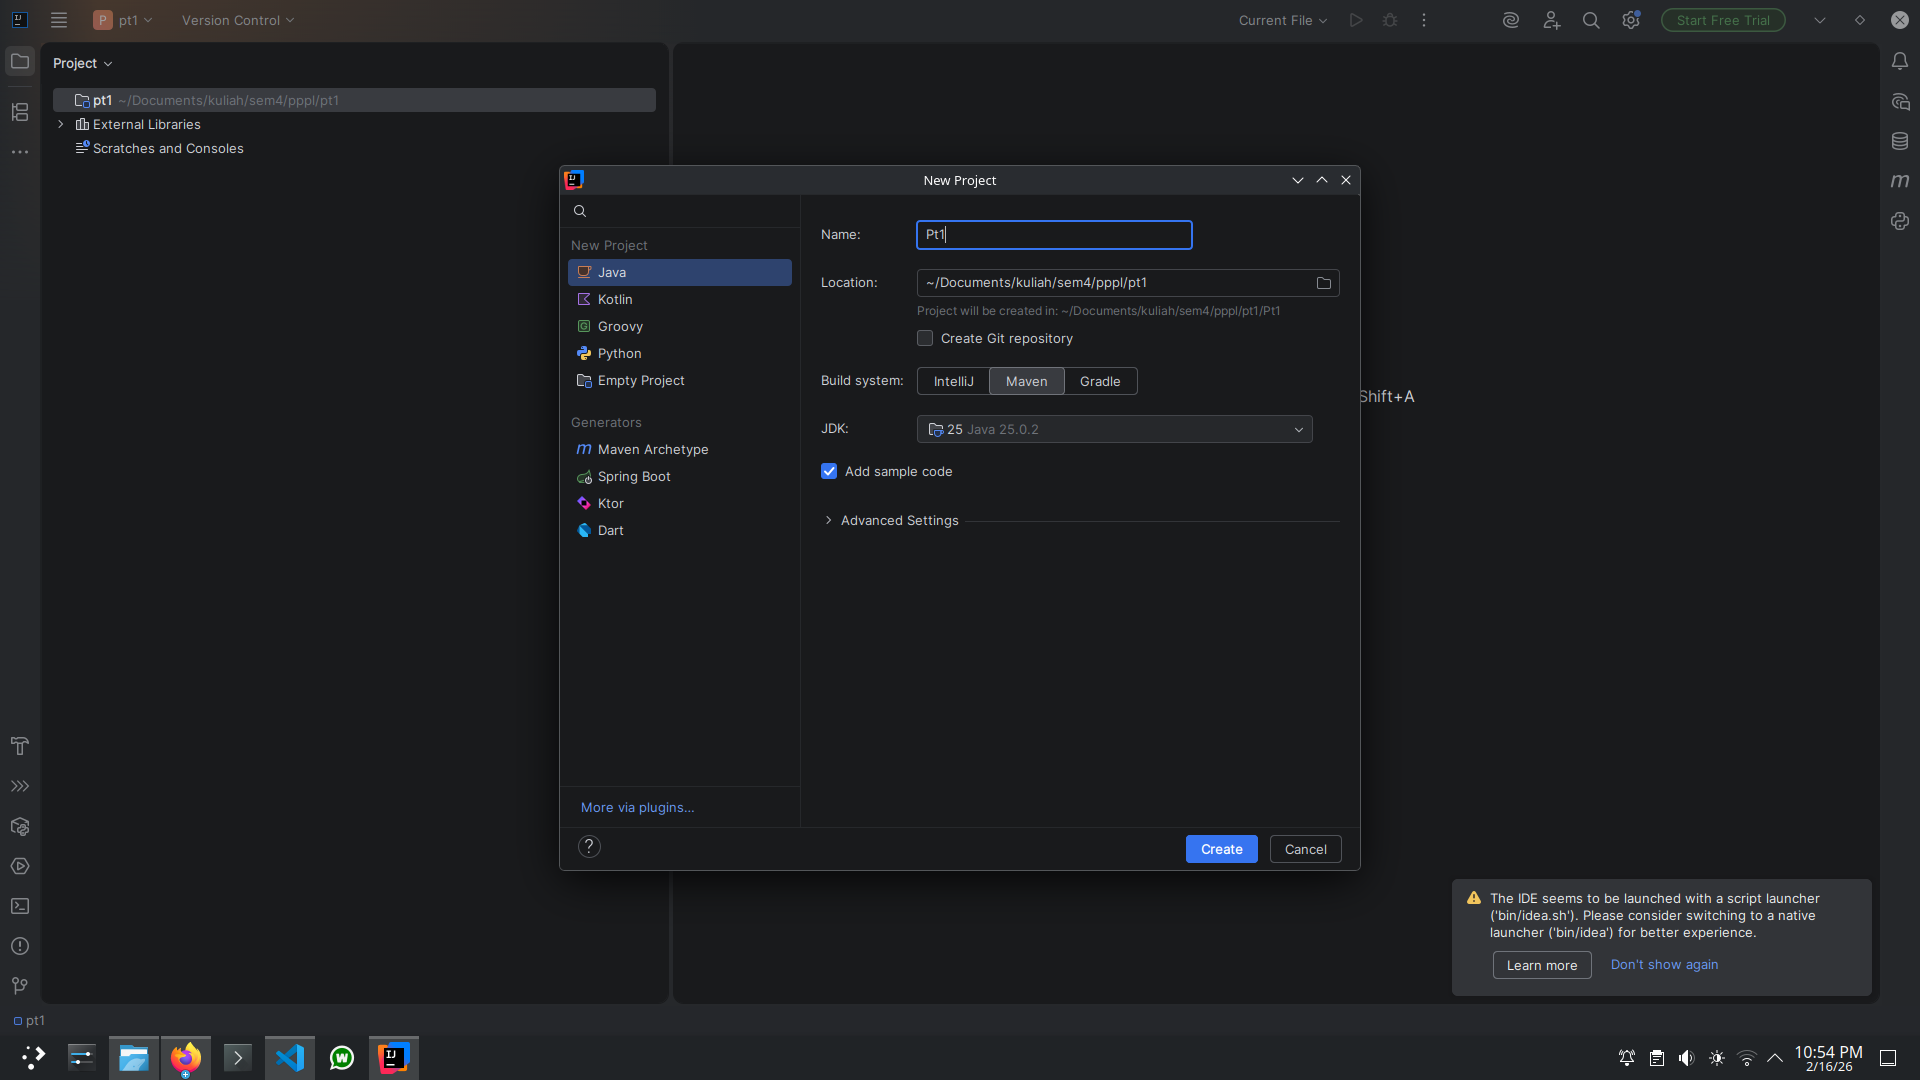
\includegraphics[width=0.8\textwidth]{one.png}
    \caption{Intellij IDEA - Proyek Maven Pt1}
\end{figure}

Kemudian, mahasiswa menambahkan dependensi JUnit Jupiter (Aggregator) ke dalam file pom.xml untuk memastikan semua komponen yang diperlukan untuk pengujian unit tersedia.
\begin{lstlisting}[style=xmlstyle]
<?xml version="1.0" encoding="UTF-8"?>
<project xmlns="http://maven.apache.org/POM/4.0.0"
         xmlns:xsi="http://www.w3.org/2001/XMLSchema-instance"
         xsi:schemaLocation="http://maven.apache.org/POM/4.0.0 http://maven.apache.org/xsd/maven-4.0.0.xsd">
    <modelVersion>4.0.0</modelVersion>

    <groupId>org.example</groupId>
    <artifactId>Pt1</artifactId>
    <version>1.0-SNAPSHOT</version>

    <properties>
        <maven.compiler.source>25</maven.compiler.source>
        <maven.compiler.target>25</maven.compiler.target>
        <project.build.sourceEncoding>UTF-8</project.build.sourceEncoding>
    </properties>

    <dependencies>
        <!-- Source: https://mvnrepository.com/artifact/org.junit.jupiter/junit-jupiter -->
        <dependency>
            <groupId>org.junit.jupiter</groupId>
            <artifactId>junit-jupiter</artifactId>
            <version>6.0.1</version>
            <scope>test</scope>
        </dependency>
    </dependencies>

</project>
\end{lstlisting}

Setelah menambahkan dependensi, mahasiswa melakukan sinkronisasi proyek untuk memastikan bahwa semua library yang diperlukan diunduh dan tersedia untuk pengembangan serta pengujian.

\vspace{2cm}

Mahasiswa diminta untuk mengerjakan tugas:

2.4 Tugas
Sebuah kelas Wallet memiliki :
\begin{enumerate}
    \item attribut owner
    \item atribut berupa list kartu-kartu
    \item atrribut untuk menyimpan list uang lembaran dan koin
    \item Fungsionalitas untuk :
\end{enumerate}
Set data owner, menambahkan kartu, mengambil kartu, menambahkan uang rupiah, mengambil uang, menampilkan jumlah uang yang ada di dompet. Implementasikan kelas tersebut dan buatlah unit testing yang sesuai dengan fungsionalitas di atas. Manfaatkanlah berbagai macam assertion yang sudah dipelajari. Method yang diimplementasikan juga bisa ditambahkan sesuai dengan kebutuhan.

Jawaban:

Struktur direktori proyek Maven yang dibuat untuk tugas ini adalah sebagai berikut:
\begin{verbatim}
Pt1 tree
.
|-- pom.xml
|-- src
|   |-- main
|   |   |-- java
|   |   |   `-- org
|   |   |       `-- example
|   |   |           |-- Card.java
|   |   |           `-- Wallet.java
|   |   `-- resources
|   `-- test
|       `-- java
|           `-- org
|               `-- example
|                   `-- WalletTest.java
`-- target
    |-- classes
    |   `-- org
    |       `-- example
    |           |-- Card.class
    |           |-- Main.class
    |           `-- Wallet.class
    |-- generated-sources
    |   `-- annotations
    |-- generated-test-sources
    |   `-- test-annotations
    `-- test-classes
        `-- org
            `-- example
                `-- WalletTest.class

22 directories, 8 files
\end{verbatim}

Terdapat 3 file utama yang digunakan untuk tugas ini, yaitu:

\subsection{Card.java}
\begin{lstlisting}[style=javastyle]
package org.example;

public class Card {
    private String namaBank;
    private String nomorRekening;

    public Card(String namaBank, String nomorRekening) {
        this.namaBank = namaBank;
        this.nomorRekening = nomorRekening;
    }

    public String getNamaBank() {
        return namaBank;
    }

    public String getNomorRekening() {
        return nomorRekening;
    }
}
\end{lstlisting}

\begin{sloppypar}
    \begin{enumerate}
        \item package org.example; untuk mendefinisikan namespace dari kelas Card, yang berada dalam paket org.example.
        \item Deklarasi kelas Card dengan dua atribut private: namaBank (nama bank penerbit kartu) dan nomorRekening (nomor rekening yang terkait dengan kartu).
        \item Konstruktor Card untuk menginisialisasi atribut namaBank dan nomorRekening saat objek Card dibuat.
        \item Getter getNamaBank() untuk mengakses nilai namaBank.
        \item Getter getNomorRekening() untuk mengakses nilai nomorRekening.
    \end{enumerate}
\end{sloppypar}
    
\subsection{Wallet.java}
\begin{lstlisting}[style=javastyle]
package org.example;

import java.util.ArrayList;
import java.util.List;

public class Wallet {
    private String owner;
    private List<Card> cards;
    private List<Integer> moneys;

    public Wallet(String owner) {
        this.owner = owner;
        this.cards = new ArrayList<>();
        this.moneys = new ArrayList<>();
    }

    public void setOwner(String owner) {
        this.owner = owner;
    }

    public String getOwner() {
        return owner;
    }

    public void addCard(String bank, String nomor) {
        Card newCard = new Card(bank, nomor);
        this.cards.add(newCard);
    }

    public Card takeCard(String nomor) {
        for (Card card : cards) {
            if (card.getNomorRekening().equals(nomor)) {
                cards.remove(card);
                return card;
            }
        }
        return null;
    }

    public List<Card> getCards() {
        return cards;
    }

    public void addMoney(Integer lembaran) {
        if (lembaran > 0) {
            this.moneys.add(lembaran);
        }
    }

    public boolean takeMoney(Integer lembaran) {
        if (this.moneys.contains(lembaran)) {
            this.moneys.remove(lembaran);
            return true;
        }
        return false;
    }

    public int calculateTotalBalance() {
        int total = 0;
        for (Integer uang : this.moneys) {
            total += uang;
        }
        return total;
    }

    public List<Integer> getMoneys() {
        return moneys;
    }
}
\end{lstlisting}

\begin{sloppypar}
    \begin{enumerate}
        \item `package` dan `import`: Menentukan paket `org.example` dan mengimpor `ArrayList`/`List` untuk struktur data.
        \item Atribut kelas: `owner` (pemilik), `cards` (list objek `Card`), dan `moneys` (list pecahan uang sebagai `Integer`).
        \item Konstruktor: Menginisialisasi `owner` serta membuat instance kosong untuk `cards` dan `moneys`.
        \item Operasi kartu: `addCard(...)` menambah `Card`; `takeCard(...)` mencari berdasarkan nomor, menghapus dan mengembalikan `Card` (atau `null`). `getCards()` mengembalikan daftar kartu.
        \item Operasi uang: `addMoney(...)` menambahkan lembaran positif; `takeMoney(...)` menghapus pecahan jika ada dan mengembalikan `boolean` keberhasilan; `calculateTotalBalance()` menjumlahkan semua pecahan.
        \item Getter tambahan: `getOwner()`/`setOwner()` dan `getMoneys()` untuk akses data.
    \end{enumerate}
\end{sloppypar}

\subsection{WalletTest.java}
\begin{lstlisting}[style=javastyle]
package org.example;

import org.junit.jupiter.api.Test;
import org.junit.jupiter.api.DisplayName;
import static org.junit.jupiter.api.Assertions.*;

class WalletTest {

    @Test
    @DisplayName("Test Inisialisasi Wallet dan Owner")
    void testWalletOwner() {
        Wallet dompet = new Wallet("Budi");
        assertNotNull(dompet, "Objek dompet tidak boleh null");
        assertEquals("Budi", dompet.getOwner());
        dompet.setOwner("Andi");
        assertEquals("Andi", dompet.getOwner());
    }

    @Test
    @DisplayName("Test Menambah dan Mengambil Kartu")
    void testCardOperations() {
        Wallet dompet = new Wallet("Siti");

        dompet.addCard("BCA", "111-222");
        dompet.addCard("Mandiri", "333-444");
        assertEquals(2, dompet.getCards().size());
        Card diambil = dompet.takeCard("111-222");

        assertAll("Verifikasi Kartu",
                () -> assertNotNull(diambil),
                () -> assertEquals("BCA", diambil.getNamaBank()),
                () -> assertEquals("111-222", diambil.getNomorRekening())
        );

        assertEquals(1, dompet.getCards().size());
    }

    @Test
    @DisplayName("Test Tambah Uang dan Hitung Total")
    void testAddMoney() {
        Wallet dompet = new Wallet("Joko");
        assertEquals(0, dompet.calculateTotalBalance());

        dompet.addMoney(10000);
        dompet.addMoney(5000);
        dompet.addMoney(500);

        assertEquals(15500, dompet.calculateTotalBalance());
    }

    @Test
    @DisplayName("Test Mengambil Uang (Withdraw)")
    void testTakeMoney() {
        Wallet dompet = new Wallet("Lina");
        dompet.addMoney(50000);
        dompet.addMoney(20000);

        boolean isSuccess = dompet.takeMoney(20000);

        assertTrue(isSuccess, "Harusnya berhasil mengambil uang yang tersedia");
        assertEquals(50000, dompet.calculateTotalBalance(), "Sisa saldo harus 50.000");

        boolean isFail = dompet.takeMoney(100000);

        assertFalse(isFail, "Harusnya gagal mengambil uang yang tidak ada");
        assertEquals(50000, dompet.calculateTotalBalance(), "Saldo tidak boleh berubah jika gagal");
    }
}
\end{lstlisting}

\begin{sloppypar}
    \begin{enumerate}
        \item `package` dan `import` JUnit 5 (`@Test`, `@DisplayName`, dan `Assertions`).
        \item Deklarasi kelas `WalletTest` yang mengelompokkan semua kasus uji untuk `Wallet`.
        \item `testWalletOwner()`: Memverifikasi inisialisasi objek dan `get/setOwner()` menggunakan `assertNotNull` dan `assertEquals`.
        \item `testCardOperations()`: Menguji `addCard()` dan `takeCard()`; menggunakan `assertEquals` untuk ukuran daftar dan `assertAll` untuk mengelompokkan beberapa pemeriksaan pada objek `Card`.
        \item `testAddMoney()`: Mengetes `addMoney()` dan `calculateTotalBalance()` (saldo awal 0 dan penjumlahan setelah penambahan).
        \item `testTakeMoney()`: Memvalidasi pengambilan uang yang berhasil dan gagal (`assertTrue`/`assertFalse`) serta memastikan saldo konsisten.
        \item Catatan: Setiap test diberi `@DisplayName` untuk keterbacaan hasil tes; kombinasi `assertAll` dan assertions individual memberikan laporan kegagalan yang informatif.
    \end{enumerate}
\end{sloppypar}

Kode dites dan menghasilkan output yang menunjukkan semua tes berhasil (green bar) tanpa kegagalan, menandakan bahwa implementasi `Wallet` telah memenuhi semua skenario pengujian yang dirancang.

\begin{figure}[h]
    \centering
    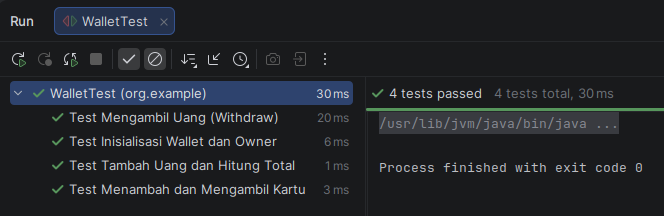
\includegraphics[width=0.8\textwidth]{testsuccess.png}
    \caption{Hasil tes JUnit menunjukkan sukses}
\end{figure}

\subsection{GitHub Repository}
Kode sumber praktikum ini dapat diakses di: \url{https://github.com/bukunya/PPPL/tree/Pertemuan1}

\section{Kesimpulan}
\begin{sloppypar}
Berdasarkan teori, implementasi, dan pengujian yang dilakukan pada praktikum ini dapat disimpulkan bahwa JUnit 6 menyediakan kerangka kerja pengujian unit yang modular dan fleksibel (Platform, Jupiter). Penggunaan assertion seperti `assertEquals`, `assertTrue`, `assertNotNull`/`assertNull` serta konstruk `assertAll` memudahkan verifikasi perilaku unit dan memberikan pelaporan kegagalan yang informatif. Implementasi kelas `Wallet` memenuhi fungsionalitas yang diminta (manajemen owner, kartu, penambahan/pengambilan uang, perhitungan saldo) dan divalidasi melalui serangkaian unit test di `WalletTest`.
\end{sloppypar}

Hasil pengujian menunjukkan kasus-kasus uji yang dirancang berjalan sukses, yang meningkatkan keandalan dan mempermudah perawatan kode. Secara keseluruhan, praktikum ini menegaskan pentingnya pengujian unit dalam menjaga kualitas perangkat lunak dan memudahkan proses pengembangan lanjutan.
\end{document}